\scanpage{162}
\margin{162}
\figure{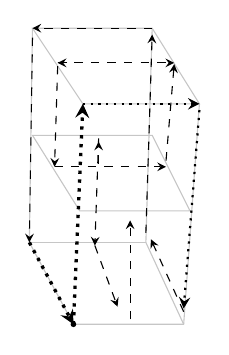
\begin{tikzpicture}[x=.8cm,y=.8cm,>=stealth]
\draw[gray!45] (0,4.7)--(1.9,4.7)--(2.65,3.5)--(.8,3.5)--cycle;
\draw[gray!45] (0,4.7)--(-.05,1.3)--(.65,0)--(2.4,0)--(2.65,3.5);
\draw[gray!45] (1.9,4.7)--(1.8,1.3)--(2.4,0);
\draw[gray!45] (0,3)--(1.9,3)--(2.5,1.8)--(.75,1.8)--cycle;
\draw[gray!45] (-.05,1.3)--(1.8,1.3);
\draw[->,dashed] (1.9,4.7)--(0,4.7); \draw[->,dashed] (0,4.55)--(-.05,1.3);
\draw[->,dashed] (1.8,1.45)--(1.9,4.6);
\draw[->,dashed] (.4,4.15)--(2.25,4.15); \draw[->,dashed] (.55,4.15)--(.4,4.15);
\draw[->,dashed] (.4,4.1)--(.35,2.5); \draw[->,dashed] (.35,2.5)--(2.12,2.5);
\draw[->,dashed] (2.12,2.6)--(2.25,4.13);
\draw[->,dotted,very thick] (-.05,1.3)--(.65,0);
\draw[->,dotted,very thick] (.65,0)--(.8,3.5); \draw[->,dotted,thick] (.8,3.5)--(2.65,3.5);
\draw[->,dotted,thick] (2.65,3.4)--(2.4,.25);
\draw[->,dashed] (1.05,2.95)--(.99,1.25); \draw[->,dashed] (1.05,2.55)--(1.05,2.9);
\draw[->,dashed] (.99,1.25)--(1.35,.28); \draw[->,dashed] (1.55,.08)--(1.55,1.65);
\draw[->,dashed] (2.4,.2)--(1.88,1.35);
\fill (.65,0) circle (.045);
\end{tikzpicture}}

\figure{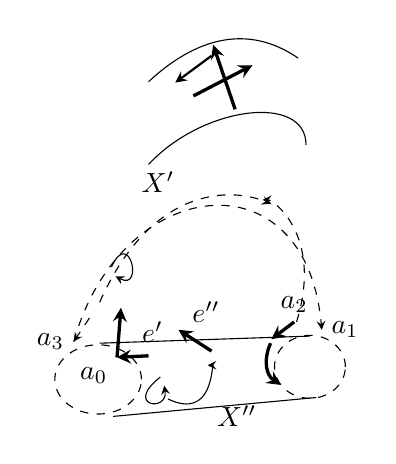
\begin{tikzpicture}[x=1cm,y=1cm,>=stealth]
\draw (-.7,3.45) .. controls (0,4.1) and (.65,4.13) .. (1.2,3.75);
\draw (-.7,2.4) .. controls (0,3.15) and (1.3,3.3) .. (1.3,2.65);
\draw[->,very thick] (.4,3.1)--(.12,3.92);
\draw[->,thick] (.1,3.78)--(-.36,3.44); \draw[->,very thick] (-.13,3.27)--(.62,3.66);
\draw[dashed,->] (-1.65,.15) .. controls (-1.05,2.28) and (1.3,2.55) .. (1.5,.3);
\draw[dashed,->] (-1.32,.65) .. controls (-.65,2.16) and (.38,2.1) .. (.85,1.9);
\draw[dashed,->] (1.18,.4) .. controls (1.52,1.5) and (.88,1.95) .. (.75,1.95);
\draw[dashed,->] (-1.45,.45)--(-1.65,.15);
\draw[dashed] (-1.34,-.33) ellipse (.55 and .44); \draw[dashed] (1.35,-.17) ellipse (.45 and .4);
\draw (-1.32,.13)--(1.35,.22); \draw (-1.15,-.8)--(1.43,-.56);
\draw[->,very thick] (-.7,-.03)--(-1.1,-.05); \draw[->,very thick] (-1.1,-.05)--(-1.05,.58);
\draw[->,very thick] (.1,.03)--(-.32,.3); \draw[->,very thick] (1.15,.4)--(.86,.18);
\draw[->,very thick] (.85,.13) .. controls (.75,-.1) and (.8,-.28) .. (.98,-.4);
\draw[->] (-.45,-.58) .. controls (.12,-.85) and (.1,-.15) .. (.05,-.15);
\draw[->] (-.55,-.3) .. controls (-1.02,-.67) and (-.45,-.75) .. (-.5,-.41);
\draw[->] (-1.17,1.1) .. controls (-.94,1.6) and (-.76,.79) .. (-1.12,.98);
\node at (-.58,2.18) {$X'$}; \node at (.42,-.8) {$X''$};
\node[left] at (-1.65,.15) {$a_3$}; \node[below left] at (-1.1,-.05) {$a_0$};
\node[above] at (1.15,.4) {$a_2$}; \node[right] at (1.5,.3) {$a_1$};
\node[above] at (-.65,.01) {$e'$}; \node[above] at (.03,.27) {$e''$};
\end{tikzpicture}}

\[
X'_{\unsure{\varepsilon|s}}\qquad X''_{\unsure{\varepsilon|s}}
\]
\diagram{\[
\left.\begin{array}{ccc}
\varepsilon_0(\unsure{X'|X}) &\xrightarrow{\sim}& \varepsilon_1(X'')\\
\varepsilon_1(X') &\xleftarrow{\sim}& \varepsilon_0(X'')
\end{array}\right\}\quad\Downarrow
\]}
\rule{5.8cm}{.4pt}
\diagram{\begin{tikzcd}[column sep=small,row sep=small]
\omega(X')\arrow[rr,no head,"\simeq"]\arrow[dr] && \omega(X'')\arrow[dl]\\
&\overset{\ominus}{\omega(X'\wedge X'')}&\begin{gathered}\text{anticommu-}\\\text{tatif}\end{gathered}
\end{tikzcd}}

$\tau',\tau'',\sigma$ ne dépendent que du ``\unsure{carré|cône} d'orientations''

$e',\ e''$ fixent les 1-orientations et aussi une \unsure{2-orientation|2-orientations} sur \uuline{chaque} \uline{morceau} $X',X''$, d'où $\rho',\rho''$
\[
\begin{array}{ll}
\tau'e'=e' & \tau''e'=-e'\\
\tau'e''=-e'' & \tau''e''=+e''
\end{array}
\]
\figure{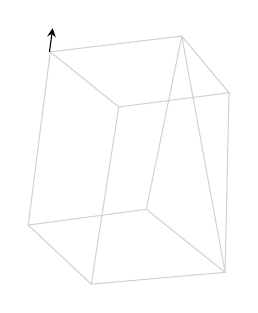
\begin{tikzpicture}[x=1cm,y=1cm,>=stealth]
\draw[gray!35] (0,0)--(1.5,.2)--(2.5,-.6)--(.8,-.75)--cycle;
\draw[gray!35] (0,0)--(.28,2.2)--(1.95,2.4)--(2.5,-.6);
\draw[gray!35] (1.5,.2)--(1.95,2.4); \draw[gray!35] (.8,-.75)--(1.15,1.5)--(2.55,1.68)--(1.95,2.4);
\draw[gray!35] (.28,2.2)--(1.15,1.5); \draw[gray!35] (2.55,1.68)--(2.5,-.6);
\draw[->] (.27,2.2)--(.31,2.5);
\end{tikzpicture}}

d'où $\rho',\rho''$
\[
\left\{\begin{array}{l}
\tau'(\rho')=\tau''(\rho')=\rho^{\prime-1}\\
\tau^{\unsure{''|'}}(\rho'')=\tau''(\rho'')=\rho^{\prime\prime-1}\\
\sigma(\rho')=\rho'',\quad\sigma\rho''=\rho'
\end{array}\right.
\]
\margin{$\begin{aligned}\rho'(e')&=e'\\\rho'(e'')&=-e'+e''\end{aligned}$}

\margin{M. \uline{Grothendieck}}
